\section{Tracking detectors \label{sec:tracking}}
\subsection[Central drift chamber]{Central drift chamber \label{sec:cdc}}

The Central Drift Chamber (CDC) is a cylindrical straw-tube drift chamber which is used to track charged particles by providing position, timing and energy loss measurements~\cite{VanHaarlem:2010yq,GlueXCDCNIM}.
The CDC is situated inside the Barrel Calorimeter, surrounding the target and Start Counter. 
The active volume of the CDC is traversed
by particles coming from the hydrogen target with polar angles between $6^{\circ}$ and $168^{\circ}$, with optimum 
coverage for polar angles between $29^{\circ}$ and $132^{\circ}$.  
The CDC contains 3522 anode wires of 20~$\mu$m diameter gold-plated tungsten inside Mylar\footnote{www.mylar.com} straw tubes of diameter 1.6~cm in $28$ layers,
located in a cylindrical volume which is 1.5~m long, with an inner radius of 10~cm and outer radius of 56~cm, as measured from the beamline.  
Readout is from the upstream end. 
Fig.\,\ref{fig:CDC_schematic} shows a schematic diagram of the detector.

\begin{figure}[tbp]
\begin{center}
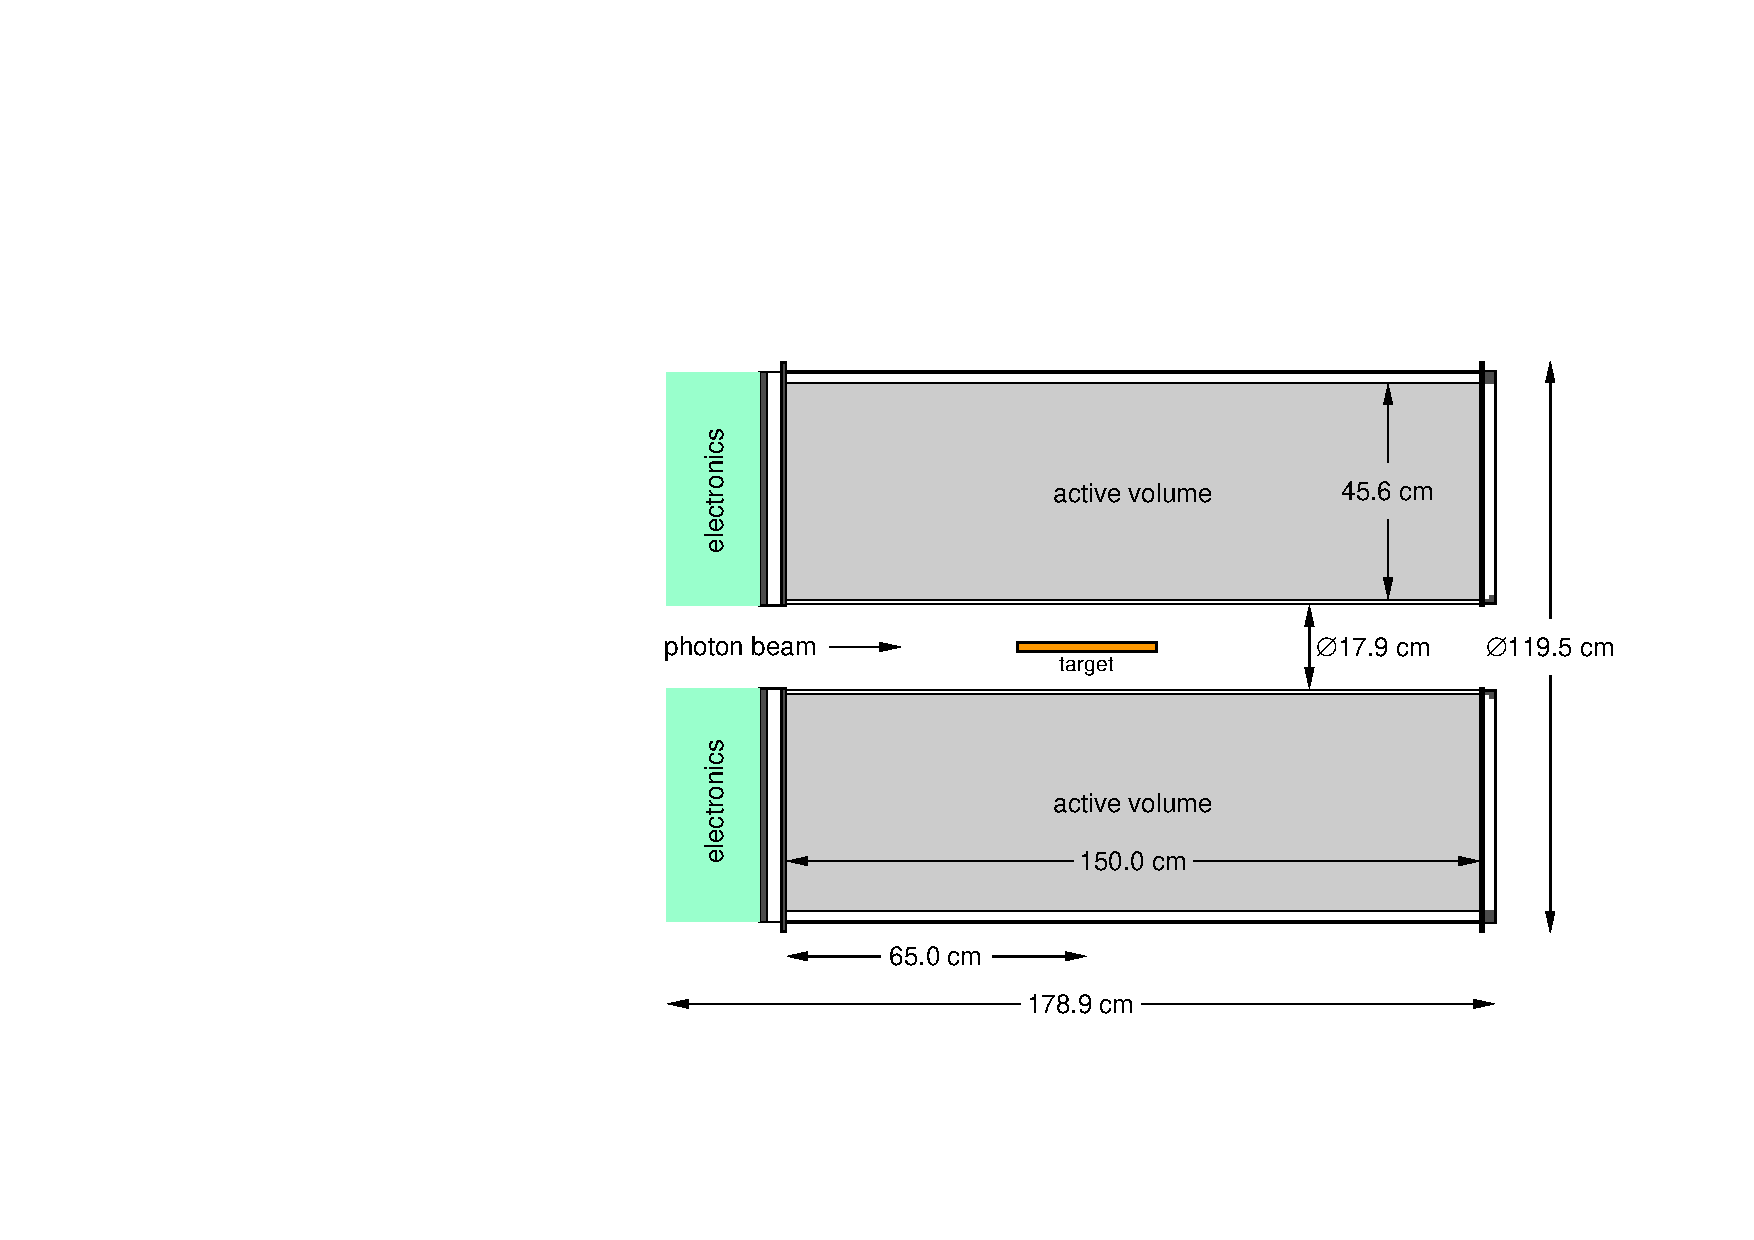
\includegraphics[width=0.7\textwidth]{figures/CDC_schematic.pdf}  
\caption{\label{fig:CDC_schematic}          
  Cross-section through the cylindrically symmetric Central Drift Chamber, along the beamline.}  
\end{center}
\end{figure}

The straw tubes are arranged in 28 layers; 12 layers are axial, and 16 layers are at stereo angles of $\pm 6^{\circ}$ to provide position information along the beam direction.
The stereo angle was chosen to balance the extra tracking information provided by the unique combination of stereo and axial straws along a trajectory against the size of the unused volume inside the chamber at each transition between stereo and axial layers. 
Fig.\,\ref{fig:CDC_stereotubes} shows the CDC during construction. 

\begin{figure}[tbp]
\begin{center}
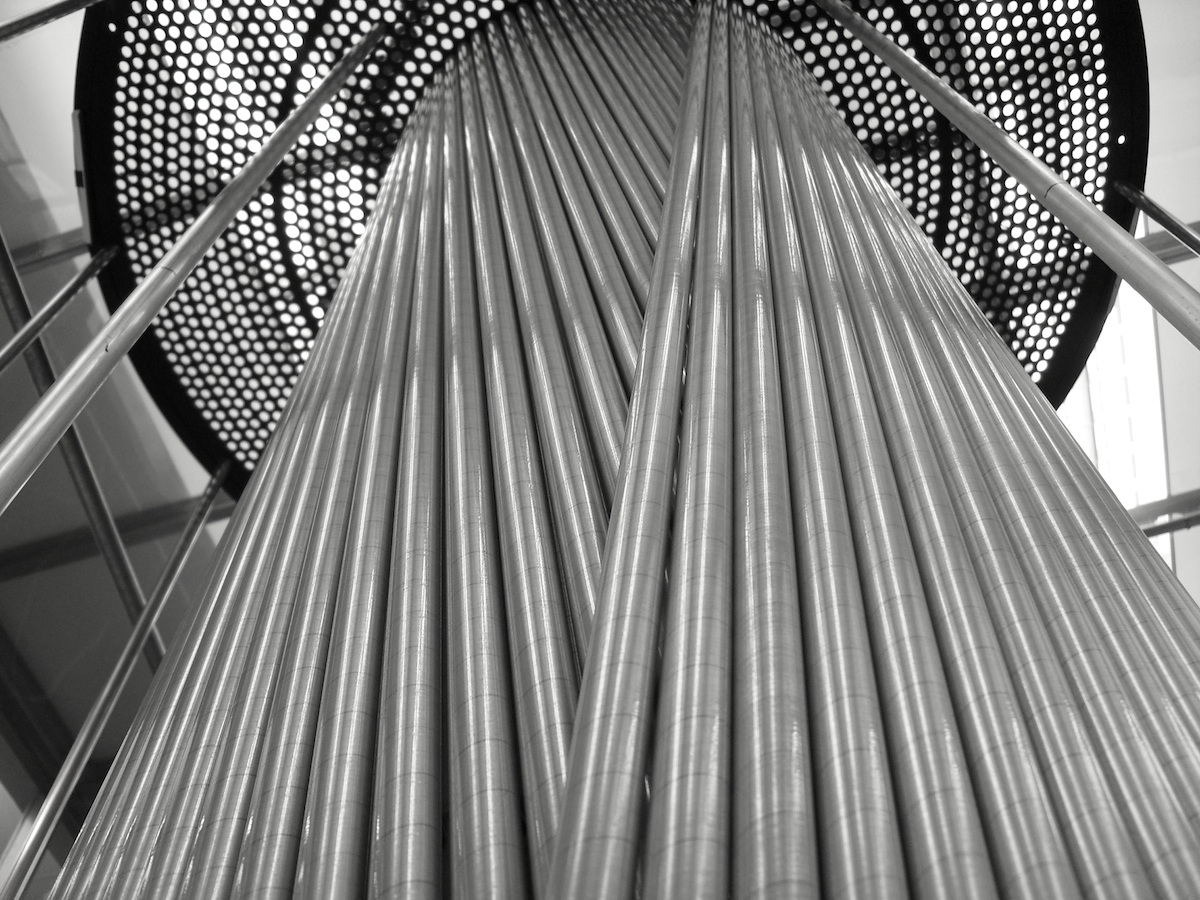
\includegraphics[width=0.7\textwidth]{figures/CDC_stereotubes.jpg}  
\caption{\label{fig:CDC_stereotubes}          
  The Central Drift Chamber during construction. A partially completed layer of stereo straw tubes is shown, surrounding a layer of straw tubes at the opposite stereo angle. Part of the carbon fiber endplate, two temporary tension rods and some of the 12 permanent support rods linking the two endplates can also be seen.}  
\end{center}
\end{figure}

The volume surrounding the straws is enclosed by an inner cylindrical wall of 0.5\,mm G10 fiberglass, an outer cylindrical wall of 1.6\,mm aluminum, and two circular endplates. 
The upstream endplate is made of aluminum, while the downstream endplate is made of carbon fiber. The endplates are connected by 12 aluminum support rods. 
Holes milled through the endplates support the ends of the straw tubes, which were glued into place using several small components per tube, described more fully in~\cite{GlueXCDCNIM}.  
These components also support the anode wires, which were installed with 30~g tension.
At the upstream end, these components are made of aluminum and were glued in place using conductive epoxy\footnote{TIGA 920-H, www.loctite.com}. 
This attachment method provides a good electrical connection to the inside walls of the straw tubes, which are coated in aluminum.
The components at the downstream end are made of Noryl plastic\footnote{www.sabic.com} and were glued in place using conventional non-conductive epoxy\footnote{3M Scotch-Weld DP460NS, www.3m.com}.
The materials used for the downstream end were chosen to be as lightweight as feasible so as to minimize the energy loss of charged particles passing through them. 

At each end of the chamber, a cylindrical gas plenum is located outside the endplate.  
The gas supply runs in 12 tubes through the volume surrounding the straws into the downstream plenum. 
There the gas enters the straws and flows through them into the upstream plenum. From the upstream plenum the gas flows into the volume surrounding the straws, and from there the gas exhausts to the outside, bubbling through small jars of mineral oil.
The gas mixture used is 50$\%$ argon and 50$\%$ carbon dioxide at atmospheric pressure. 
This gas mixture was chosen since its drift time characteristics provide good position resolution~\cite{VanHaarlem:2010yq}.
A small admixture (approximately 1$\%$) of isopropanol is used to prevent loss of performance due to aging\cite{KADYK1991436,VAVRA20031}. 
Five thermocouples are located in each plenum and used to monitor the temperature of the gas.
The downstream plenum is 2.54~cm deep, with a sidewall of ROHACELL\footnote{www.rohacell.com} and a final outer wall of aluminized Mylar film, and the upstream plenum is 3.18~cm deep, with a polycarbonate sidewall and a polycarbonate disc outer wall. 

The readout cables pass through the polycarbonate disc and the upstream plenum to reach the anode wires. 
The cables are connected in groups of 20 to 24 to transition boards mounted onto the polycarbonate disc; the disc also supports the connectors for the high-voltage boards. 
Preamplifiers~\cite{hdnote2515} are mounted on the high-voltage boards. The aluminum endplate, outer cylindrical wall of the chamber, aluminum components connecting the straws to the aluminum endplate and the inside walls of the straws are all connected to a common electrical ground. 
The anode wires are held at +2.1~kV during normal operation. 


\subsection[Forward Drift Chamber]{Forward Drift Chamber
\label{sec:fdc} }

The Forward Drift Chamber (FDC) consists of 24 disc-shaped planar drift chambers of 1~m diameter \cite{FDC_NIM}.
They are grouped into four packages inside the bore of the spectrometer magnet.
Forward tracking requires good multi-track separation due to the
high particle density in the forward region.
This is achieved via additional cathode strips on both sides of the wire plane allowing for a  reconstruction of a space point on the track from each chamber. 
The FDC registers particles emitted into polar angles as low as $1^\circ$ and up to $10^\circ $
with all the chambers, while having partial coverage up to $20^\circ$.

One FDC chamber consists of a wire plane with cathode planes on either sides at a distance of $5$~mm from the wires (Fig.~\ref{FDC_OneCell}).
\begin{figure}[tbp]
\begin{center}
%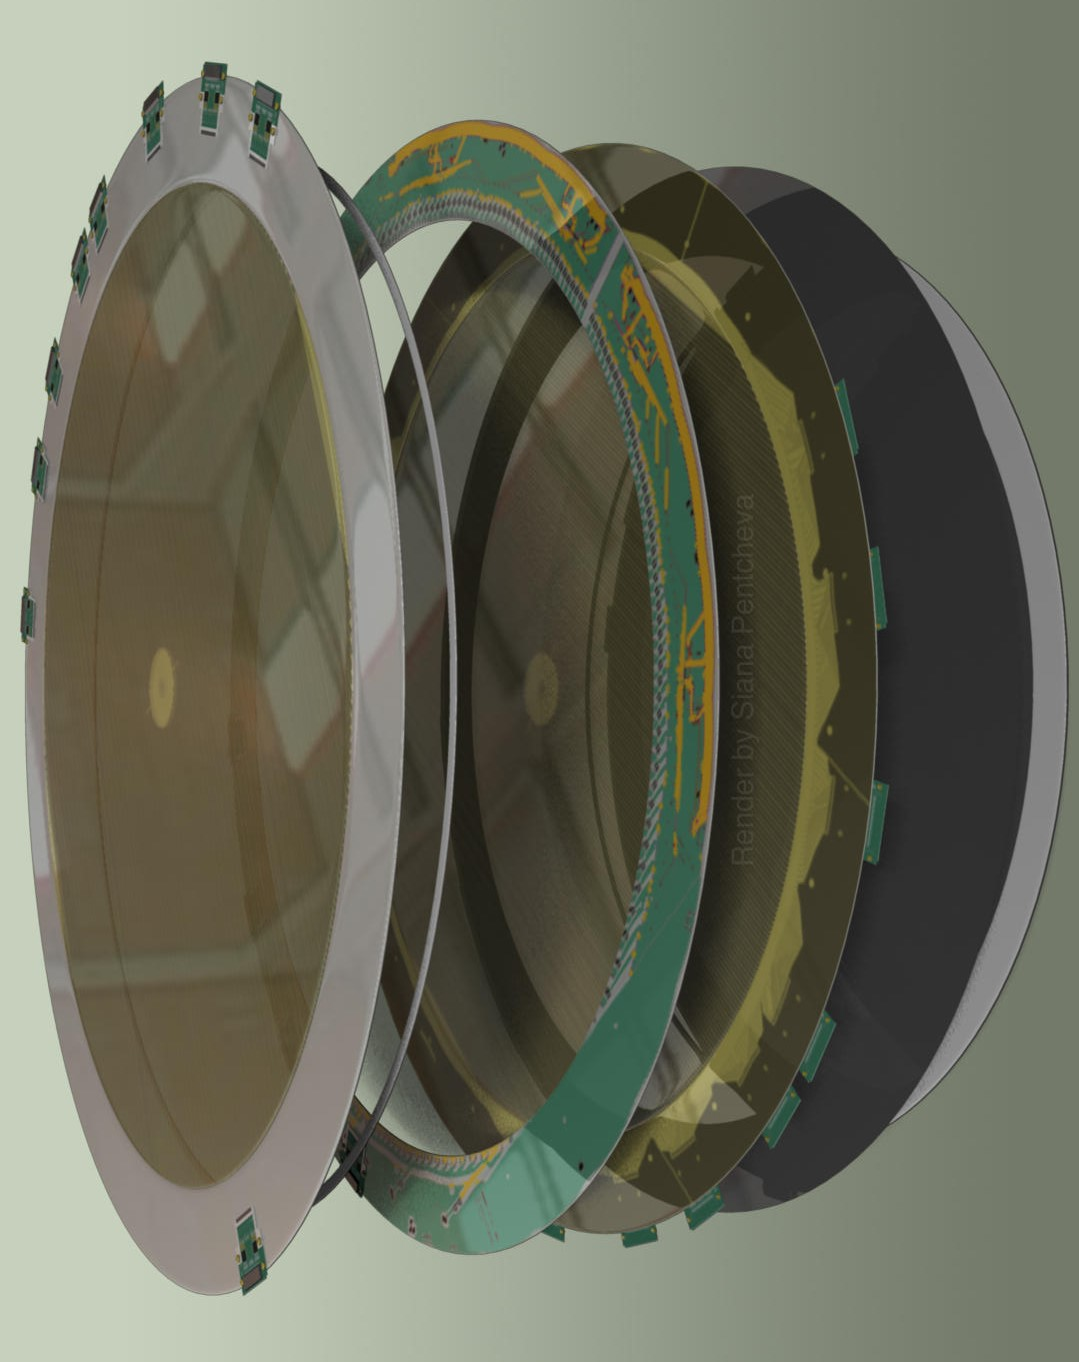
\includegraphics[width=0.75\textwidth]{figures/FDC_OneCell.jpg}  
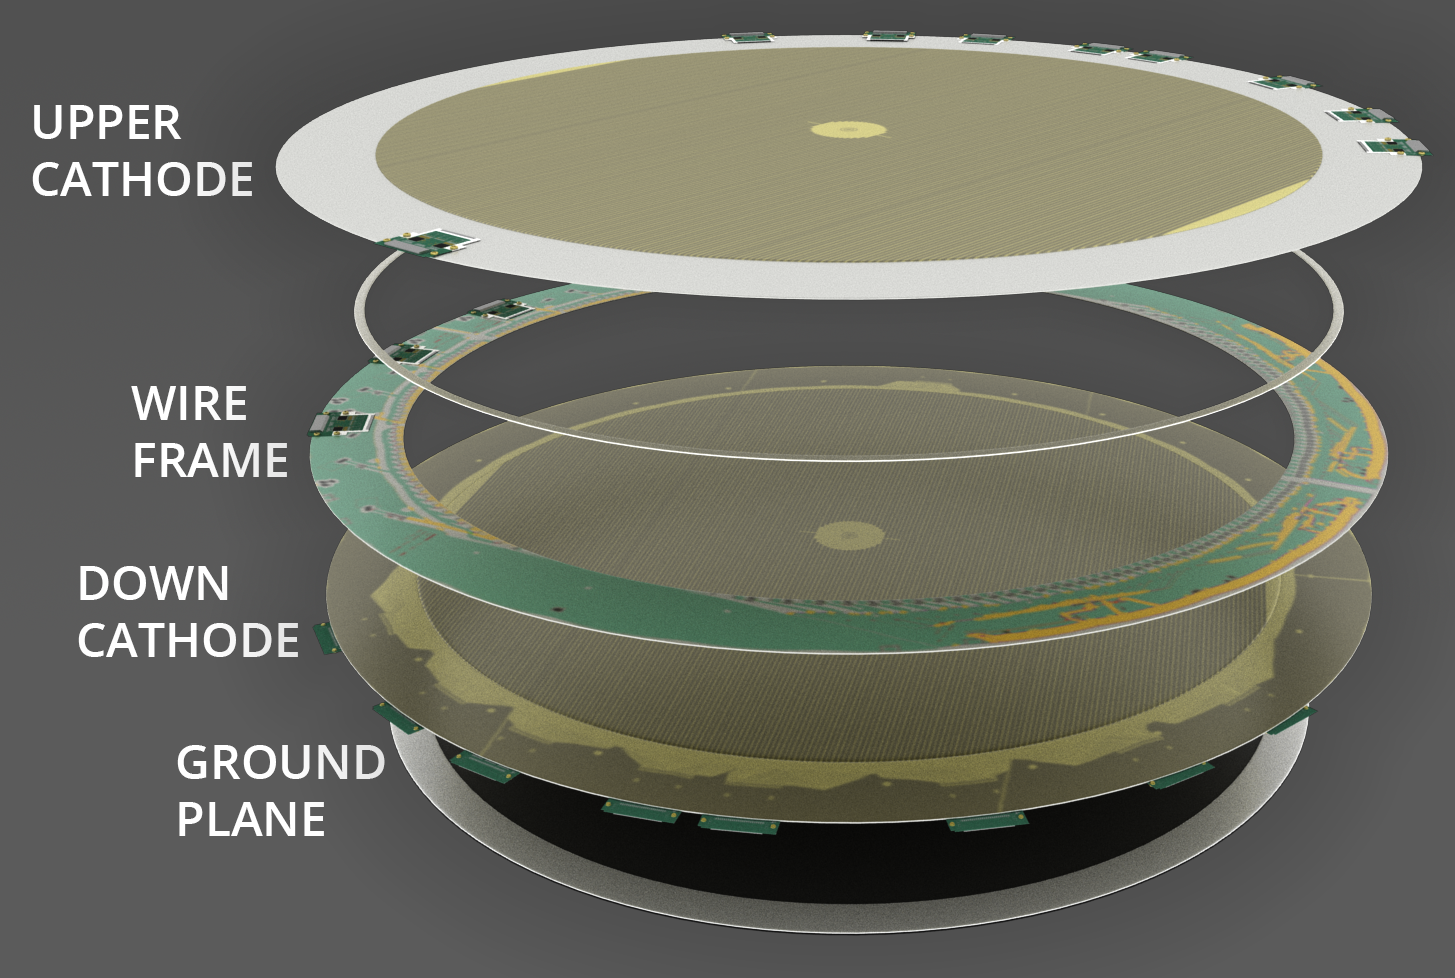
\includegraphics[width=0.95\textwidth]{figures/FDC_OneCell2.png} 
\caption{\label{FDC_OneCell}
Artist rendering of one FDC chamber showing components. From top to bottom: upstream cathode, wire frame, downstream cathode, ground plane that separates the chambers. The diameter of the active area is $1$~m.
}
\end{center}
\end{figure}
The frame that holds the wires is made out of ROHACELL with a thin
G10 fiberglass skin in order to minimize the material and
allow low energy photons to be detected in the outer electromagnetic calorimeters.

The wire plane has sense ($20~\mu$m diameter) and field ($80$~$\mu$m) wires $5$~mm apart, forming a field cell of $10\times 10$~mm$^2$. 
To reduce the effects of the magnetic field, 
a ``slow" gas mixture of $40\%$~Ar and $60\%$~CO$_2$ is used.
A positive high voltage of about $2.2$~kV is applied to the sense wires and a negative high voltage of $0.5$~kV to the field wires. 
The cathodes are made out of $2$-$\mu$m-thin copper strips on Kapton foil with a pitch of $5$~mm, and are held at ground potential. The strips on the two cathodes are arranged at $30^\circ $ relative to each other and at angles of $75^\circ $ and $105^\circ $ angle with respect to the wires.

The six chambers of a package are separated by thin aluminized Mylar.
Each chamber is rotated relative to the previous one by $60^\circ $.
The total material of a package in the sensitive area corresponds to $0.43\%$ radiation lengths, with about half of that in the area along the beam line that has no copper on the cathodes.
The sense wires in the inner area of $6-7.8$~cm diameter (depending on the distance of the package to the target) are increased in thickness from $20$~$\mu$m to $\sim 80$~$\mu$m, which makes them insensitive to the high rates along the beam.
The distance between the first and last package is $1.69$~m. 
All chambers are supplied with gas in parallel. 
In total, $2,304$ wires and $10,368$ strips are read using charge preamplifiers with $10$~ns peaking time, with a gain of $0.77$~mV/fC for the wires and $2.6$~mV/fC for the strips.

\subsection{Electronics \label{sec:dcelectronics}}
The high voltage (HV) supply units used are CAEN A1550P\footnote{www.caen.it}, with noise-reducing filter modules added to each crate chassis. 
The low voltage (LV) supplies are Wiener MPOD MPV8008\footnote{www.wiener-d.com}. 
The preamplifiers are a custom JLab design based on an ASIC~\cite{hdnote2515}
with 24 channels per board; the preamplifiers are charge-sensitive, capacitively coupled to the wires in the CDC and FDC, and directly coupled to strips in the FDC. 

Pulse information from the CDC anode wires and FDC cathode strips are obtained and read out using 72-channel 125 MHz flash ADCs (FADCs) \cite{Visser2008,5873864}. These use Xilinx\footnote{www.xilinx.com} Spartan-6 FPGAs (XC6SLX25) for signal digitization and data processing with 12 bit resolution.
Each FADC receives signals from three preamplifiers. 
The signal cables from different regions of the drift chambers are distributed between the FADCs in order to share out the processing load as evenly as possible.  

The FADC firmware is activated by a signal from the \gx{} trigger. The firmware then computes the following quantities for pulses observed above a given threshold within a given time window: pulse number, arrival time, pulse height, pulse integral, pedestal level preceding the pulse, and a quality factor indicating the accuracy of the computed arrival time. 
Signal filtering and interpolation are used to obtain the arrival time to the nearest 0.8~ns. 
The firmware performs these calculations both for the CDC and FDC alike, and uses different readout modes to provide the data with the precision required by the separate detectors. 
For example, the CDC electronics read out only one pulse but require both pulse height and integral, while the FDC electronics read out up to four pulses and do not require a pulse integral.  

The FDC anode wires are read out using the JLab pipeline F1 TDC\cite{hdnote1021} with a nominal least count of 120~ps. 

\subsection[Gas system]{Gas system \label{sec:gas}}
Both the CDC and FDC operate with the same gases, argon and CO$_{2}$. Since the relative mixture of
the two gases is slightly different for the two tracking chambers, the gas system has two separate but identical mixing stations. There is one gas supply of argon and CO$_{2}$ for both mixing stations. A limiting opening in the supply
lines provides over-pressure protection to the gas system, and filters in the gas lines provide protection against potential
pollution of the gas from the supply. Both gases are mixed using mass flow controllers (MFCs) that can be 
configured
to provide the desired mixing ratio of argon and CO$_{2}$.  MFCs and control electronics from
BROOKS Instruments\footnote{BROOKS Instruments, https://www.brooksinstrument.com/en/products/mass-flow-controllers.} are used throughout.

The mixed gas is filled into storage tanks, with one tank for the CDC and another for the FDC. The pressures are
regulated by controlling the operation of the MFCs with a logic circuit based on an Allen-Bradley ControlLogix system\footnote{Allen-Bradley, https://ab.rockwellautomation.com/}
 that keeps
the pressure in the tank between 10 and 12~psi. The tank serves both as a reservoir and a buffer.
A safety relief valve on each tank
provides additional protection against over-pressure. While the input pressure to the MFC is at 40~psi, the pressure after
the MFC is designed to always be less than 14~psi above atmospheric pressure. After the mixing tank, a provision is
built into the system to allow the gas to pass through an alcohol bath to add a small amount of alcohol gas to the gas mixture.
This small admixture of alcohol protects the wire chambers from aging effects caused by radiation exposure from the beam.
This part of the gas system is located above ground in a separate gas shed, before the gas mixture is transported
to the experimental hall via polyethylene pipes.

Additional MFCs in the hall allow the exact amount of gas provided to the chambers to be specified: one MFC for the CDC and another 
four MFCs for the individual FDC packages. The CDC is operated with a flow of 1.0~l/m, while each FDC package is operated with
a flow of 0.1~l/m. To protect the chambers from over-pressure, there is a bypass line at the input to the detectors that
is open to the atmosphere following a bubbler containing mineral oil. The height of the oil level determines the maximum possible gas pressure at
the input to the chambers. There is a second bubbler at the output to protect against possible air back-flow into
the chamber. The height of the oil above the exhaust line determines the operating pressure inside the chambers.

Valves are mounted at many locations in the gas system to monitor various pressures with a single pressure sensor. The pressures of all six FDC chambers are monitored, as well as the CDC gas at the input, downstream gas plenum and the exhaust. 
A valve in the exhaust line can be used to divert some gas from the chamber to an oxygen sensor. Trace quantities of oxygen will reduce the gas gain and reduce tracking efficiency. The oxygen levels in the chamber are below 100~ppm.

\subsection{Calibration, performance and monitoring \label{sec:dccalib}}
Time calibrations for the drift chambers are used to remove the time offset due to the electronics, so that after calibration the earliest possible arrival time of the pulse signals is at 0~ns. These offsets and the function parameters used to describe the relationship between the pulse arrival time and the closest distance between the track and the anode wire are obtained for each session of data taking. 

The CDC measures the energy loss, $dE/dx$, of tracks over a wide range of polar angles, including recoiling target protons as well as more forward-going tracks. Gain calibrations are made to ensure that $dE/dx$ is consistent between tracking paths through different straws and stable over time. 
The procedure entails matching the position of the minimum ionizing peak for each of the 3522 straws, and then matching the $dE/dx$ at 1.5~GeV/c to the calculated value of 2.0~ keV/cm. This takes place during the early stages of data analysis. Gain calibration for the individual wires is performed each time the HV is switched on and whenever any electronics modules are replaced. Gain calibration for the chamber as a whole is performed for each session of data taking; these sessions are limited to two hours as the gain is very sensitive to the atmospheric pressure. Position calibrations were necessary to describe the small deflection of the straw tubes midway along their length; these were performed in 2016 and repeated in 2017, with no significant difference found between the two sets of results.  Position resolution from the CDC is of the order of 130~$\mu$m and its detection efficiency per straw is over 98\% for tracks up to 4~mm from the CDC wire. The efficiency decreases as the distance between the track and the wire increases, but the close-packing arrangement of the straw tubes and the large number of straws traversed by each track compensate for this. 

For the FDC system, an internal per-chamber calibration process is first performed to optimize the track position accuracy.  
In the FDC the avalanche created around the wire is seen in three projections: on the two cathodes and on the wires.
The drift time information from the wires is used to reconstruct the hit position perpendicular to the wire.
The strip charges from the two cathodes are used to reconstruct the avalanche position along the wire. 
The same strip information can be used to reconstruct the avalanche position perpendicular to the wire,  which, due to the proximity of the avalanche to the wire, is practically the wire position, as illustrated in Fig~\ref{FDC_wires_from_strips}.
\begin{figure}[tbp]
\begin{center}
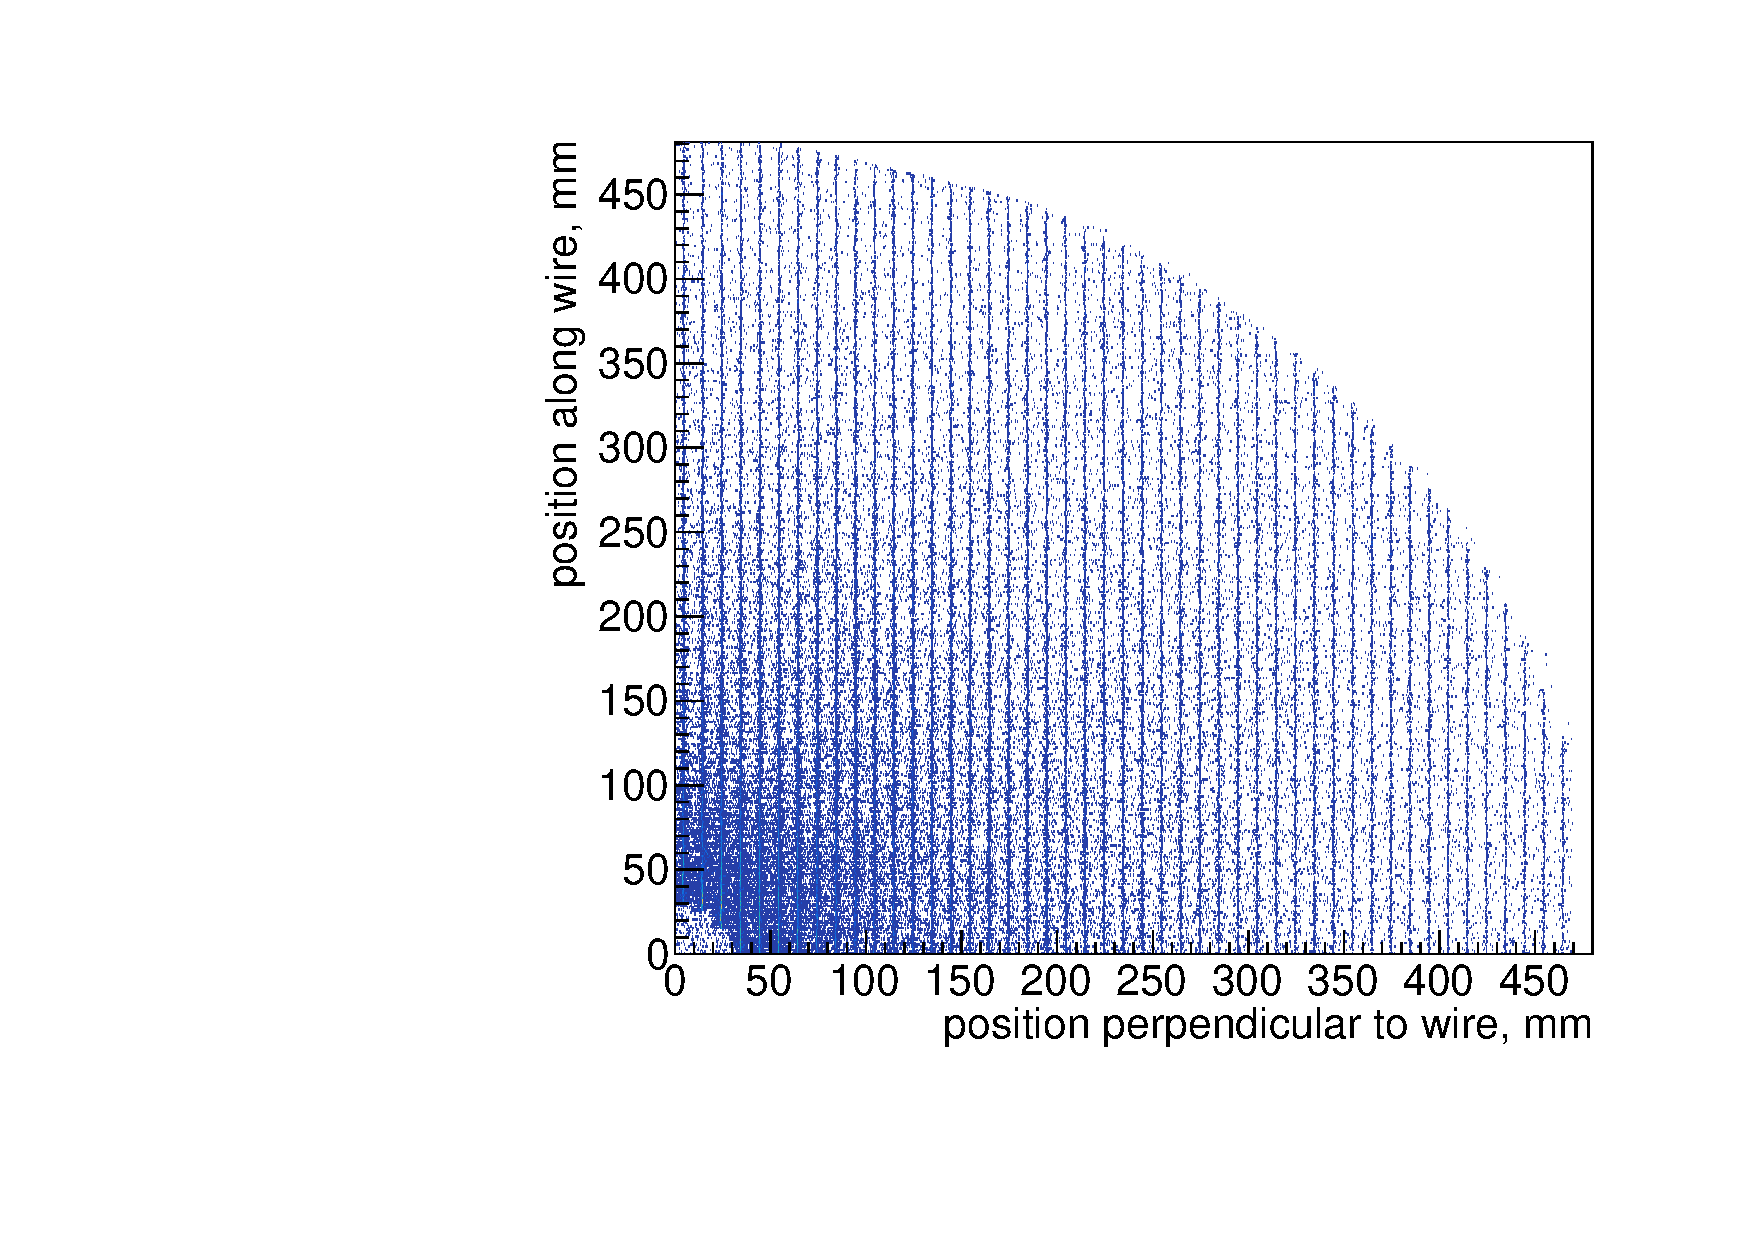
\includegraphics[width=0.95\textwidth]{figures/FDC_wires_from_strips1.pdf}  
\caption{\label{FDC_wires_from_strips} Wire (avalanche) positions reconstructed from the strip information on the two cathodes in one FDC chamber. Only one quarter of the chamber is shown in this figure.
}   
\end{center}  
\end{figure}
This strip information is used to align the strips on the two cathodes with respect to the wires. 
At the same time, the residuals of the reconstructed wire positions are an estimate of the strip resolution.
The resolutions of the detector were reported earlier \cite{FDC_NIM}. 
The strip resolution along the wires, estimated from the wire position reconstruction, varies between $180$ and $80$~$\mu$m, depending on the total charge induced on the strips. The drift distance is reconstructed from the drift time with a resolution between $240$ and $140$~$\mu$m
depending on the distance of the hit to the wire in the $0.5-4.5$~mm range.  

Position offsets and package rotations were determined for both drift chamber systems, first independently, and then together, using the alignment software MILLEPEDE\cite{millepede} in a process described in \cite{GlueXCDCNIM} and in \cite{MikeStaib_thesis}.

Online monitoring software enables shift-takers to check that the number of channels recording data, the distribution of signal arrival times, and the  $dE/dx$ distribution are as expected. 


%\subsection{Summary \label{sec:dcsummary}}
 
 
